\PassOptionsToPackage{table}{xcolor}

\documentclass[
%	handout,
	notes=none,
	aspectratio=169
]{beamer}

% Comment out the following line to hide the notes
%\setbeameroption{show notes}

% Imports
\usepackage{listings}
\usepackage{amsfonts}
\usepackage{amsmath}
\usepackage{pythonhighlight}
\usepackage{pgfpages}
\usepackage{tabularx}

\mode<handout>{%
	\pgfpagesuselayout{8 on 1}[a4paper,border shrink=5mm]
	\setbeameroption{show notes}
}

% Graphics configuration
\graphicspath{{./graphics/}}
\DeclareGraphicsExtensions{.pdf,.jpeg,.png,.jpg,.pdf}

% Useful macros
\def\etal{{\it et al.}}
\def\etc{{\it etc.}}
\def\eg{{\it e.g.}}
\def\ie{{\it i.e.}}
\def\cf{{\it cf.}}
\def\qv{{\it q.v.}}
\def\qqv{{\it qq.v.}}
\def\st{s.t.\ }
\def\code{\tt}
\def\setsep{:}
\def\concat{\mathbin{|}}

\renewcommand{\thefootnote}{\fnsymbol{footnote}}
\newcommand{\prescite}[1]{\footnote{\cite{#1}}}
\newcommand{\prestext}[1]{\footnotetext{\cite{#1}}}
\newcommand{\emaillink}[1]{\href{mailto:#1}{\nolinkurl{#1}}}

\setlength{\parskip}{0.5em}

% Tables

\newcolumntype{L}[1]{>{\raggedright\arraybackslash\tiny}p{#1}}

% Program listings
\definecolor{listingbaground}{rgb}{.9,.9,.9}

\lstset{
	language=C,
	backgroundcolor=\color{listingbaground},
	extendedchars=true,
	basicstyle=\fontsize{5pt}{6pt}\ttfamily,
	showstringspaces=false,
	showspaces=false,
	numbers=left,
	numberstyle=\fontsize{5pt}{6pt}\ttfamily\color{gray},
	numbersep=5pt,
	tabsize=2,
	breaklines=true,
	showtabs=false,
	captionpos=b,
	xleftmargin=5mm,
	escapeinside={££}{££},
	framexleftmargin=5mm
}

% https://tex.stackexchange.com/questions/89574/language-option-supported-in-listings
\lstdefinelanguage{JavaScript}{
	keywords={typeof, new, true, false, catch, function, return, null, catch, switch, var, if, in, while, do, else, case, break},
	keywordstyle=\color{blue}\bfseries,
	ndkeywords={class, export, boolean, throw, implements, import, this},
	ndkeywordstyle=\color{darkgray}\bfseries,
	identifierstyle=\color{black},
	sensitive=false,
	comment=[l]{//},
	morecomment=[s]{/*}{*/},
	commentstyle=\color{purple}\ttfamily,
	stringstyle=\color{red}\ttfamily,
	morestring=[b]',
	morestring=[b]"
}

\lstdefinelanguage{QML}{
	keywords={typeof, new, true, false, catch, function, return, null, catch, switch, var, if, in, while, do, else, case, break, id, property, bool, string, int, decimal, target},
	keywordstyle=\color{blue}\bfseries,
	ndkeywords={Page, Example, Timer, Column, PageHeader, TextSwitch, Label},
	ndkeywordstyle=\color{teal}\bfseries,
	identifierstyle=\color{black},
	sensitive=true,
	comment=[l]{//},
	morecomment=[s]{/*}{*/},
	commentstyle=\color{green}\ttfamily,
	stringstyle=\color{red}\ttfamily,
	morestring=[b]',
	morestring=[b]"
}

\lstdefinelanguage{cpp}{
	keywords={class, public, private, try, throw, catch, this, return, null, switch, if, while, do, else, case, break, for, bool, void, const},
	keywordstyle=\color{blue}\bfseries,
	ndkeywords={Q_OBJECT, Q_CLASSINFO, Q_PROPERTY, Q_SLOTS, Q_SIGNALS, signals, slots, READ, WRITE, NOTIFY},
	ndkeywordstyle=\color{teal}\bfseries,
	identifierstyle=\color{black},
	sensitive=false,
	comment=[l]{//},
	morecomment=[s]{/*}{*/},
	commentstyle=\color{purple}\ttfamily,
	stringstyle=\color{red}\ttfamily,
	morestring=[b]',
	morestring=[b]"
}

\lstdefinelanguage{sh2}{
	keywords={dbus, send, zypper, python3},
	keywordstyle=\color{blue}\bfseries,
	ndkeywords={session, type, print, reply, dest},
	ndkeywordstyle=\color{teal}\bfseries,
	identifierstyle=\color{black},
	sensitive=false,
	comment=[l]{\#},
	morecomment=[s]{/*}{*/},
	commentstyle=\color{purple}\ttfamily,
	stringstyle=\color{red}\ttfamily,
	morestring=[b]',
	morestring=[b]"
}

% To allow the theme files to be placed in a subdirectory
\makeatletter
	\def\beamer@calltheme#1#2#3{%
		\def\beamer@themelist{#2}
		\@for\beamer@themename:=\beamer@themelist\do
		{\usepackage[{#1}]{\beamer@themelocation/#3\beamer@themename}}}

	\def\usefolder#1{
		\def\beamer@themelocation{#1}
	}
	\def\beamer@themelocation{}






\usefolder{theme}
\usetheme{sailfish}

\begin{document}

\title{Running Linux on your Smartphone}
\subtitle{REG Lunchtime Tech Talk}
\author{David Llewellyn-Jones}
\date{9th May 2023}

%%%%%%%%%%%%%%%%%%%%%%%%%%%%%%%%%%%%%%%%%

\renewcommand{\thefootnote}{\arabic{footnote}}

\frame{
\titlepage
}
\note{
}

\renewcommand{\thefootnote}{\fnsymbol{footnote}}

%%%%%%%%%%%%%%%%%%%%%%%%%%%%%%%%%%%%%%%%%

\begin{frame}
\frametitle{Smartphone Operating Systems}

\begin{columns}[T]
\begin{column}[T]{0.93\textwidth}

\vspace{1.0cm}
\includegraphics[height=0.75\textheight]{android-ios}

\end{column}
\end{columns}

\end{frame}
\note{
Most users are running one of two Smartphone Operating Systems
\begin{enumerate}
\setlength{\parskip}{0.5em}
\item Android: https://betawiki.net/wiki/Android_13
\item iOS: https://betawiki.net/wiki/IOS_16.0_build_20A362
\end{enumerate}
}

%%%%%%%%%%%%%%%%%%%%%%%%%%%%%%%%%%%%%%%%%

\begin{frame}
\frametitle{Android}

\begin{columns}[T]
\begin{column}[T]{0.5\textwidth}

\vspace{1.0cm}
\hspace{2.14em}\includegraphics[height=0.75\textheight]{android}

\end{column}

\begin{column}[T]{0.5\textwidth}
\setlength{\parskip}{0.5em}

\vspace{1.7cm}
\begin{enumerate}
\setlength{\parskip}{0.5em}
\item AOSP (Android Open Source Project)
\item Linux kernel
\item GMS (Google Mobile Services)
\item Apps written in Java, Kotlin, others
\item Linux, but not as we know it
\end{enumerate}

\end{column}
\end{columns}

\end{frame}
\note{
}

%%%%%%%%%%%%%%%%%%%%%%%%%%%%%%%%%%%%%%%%%

\begin{frame}
\frametitle{iOS}

\begin{columns}[T]
\begin{column}[T]{0.5\textwidth}
\setlength{\parskip}{0.5em}

\vspace{1.7cm}
\begin{enumerate}
\setlength{\parskip}{0.5em}
\item Darwin (BSD) kernel
\item Cocoa Touch user interface
\item Apps written in Objective-C, Swift
\item Closed source, closed ecosystem
\end{enumerate}

\end{column}

\begin{column}[T]{0.5\textwidth}

\vspace{1.0cm}
\hspace{1.54em}\includegraphics[height=0.75\textheight]{ios}

\end{column}
\end{columns}

\end{frame}
\note{
}

%%%%%%%%%%%%%%%%%%%%%%%%%%%%%%%%%%%%%%%%%

\begin{frame}
\frametitle{Linux}

\begin{columns}[T]
\begin{column}[T]{0.65\textwidth}
\setlength{\parskip}{0.5em}

\vspace{1.0cm}
\begin{enumerate}
\setlength{\parskip}{0.5em}
\item Mobian (Debian + Phosh)
\item postmarketOS (Alpine Linux + Plasma Mobile)
\item Ubuntu Touch (Ubuntu + Lomiri)
\item Nemo Mobile (Manjaro + Nemo)
\item Sailfish OS (Mer + Silica)
\end{enumerate}

\end{column}
\begin{column}[T]{0.35\textwidth}

\vspace{0.0cm}

\includegraphics[height=1.2\textwidth]{variants}

\end{column}
\end{columns}

\end{frame}
\note{
}

%%%%%%%%%%%%%%%%%%%%%%%%%%%%%%%%%%%%%%%%%

\begin{frame}
\frametitle{Why are they interesting?}

\begin{columns}[T]
\begin{column}[T]{1.0\textwidth}
\setlength{\parskip}{0.5em}

\vspace{0.4cm}
\begin{enumerate}
\setlength{\parskip}{0.5em}
\item Linux, glibc, GNU Core Utils, systemd
\item Open Source
\item Open development models
\item Open ecosystems
\item Community-oriented business models
\item Most Linux software just compiles and runs
\end{enumerate}

\end{column}
\end{columns}

\end{frame}
\note{
}

%%%%%%%%%%%%%%%%%%%%%%%%%%%%%%%%%%%%%%%%%

\begin{frame}
\frametitle{Linux on Mobile History}

\begin{columns}[T]
\begin{column}[T]{1.1\textwidth}

\vspace{0.5cm}
\includegraphics[width=1.0\textwidth]{timeline}

\end{column}
\end{columns}

\end{frame}
\note{
}

%%%%%%%%%%%%%%%%%%%%%%%%%%%%%%%%%%%%%%%%%

\begin{frame}
\frametitle{Maemo 4.1}

\begin{columns}[T]
\begin{column}[T]{1.0\textwidth}

\vspace{0.5cm}
\begin{center}
\includegraphics[width=0.6\textwidth]{n810}
\end{center}

\end{column}
\end{columns}

\end{frame}
\note{
}

%%%%%%%%%%%%%%%%%%%%%%%%%%%%%%%%%%%%%%%%%

\begin{frame}
\frametitle{Maemo 5}

\begin{columns}[T]
\begin{column}[T]{1.0\textwidth}

\vspace{0.8cm}
\begin{center}
\includegraphics[width=0.6\textwidth]{n900}
\end{center}

\end{column}
\end{columns}

\end{frame}
\note{
}

%%%%%%%%%%%%%%%%%%%%%%%%%%%%%%%%%%%%%%%%%

\begin{frame}
\frametitle{Salfish OS 2.2}

\begin{columns}[T]
\begin{column}[T]{1.0\textwidth}

\vspace{0.3cm}
\begin{center}
\includegraphics[width=0.3\textwidth]{jolla1}
\end{center}

\end{column}
\end{columns}

\end{frame}
\note{
}

%%%%%%%%%%%%%%%%%%%%%%%%%%%%%%%%%%%%%%%%%

\begin{frame}
\frametitle{Jolla 1 Launch}

\begin{tikzpicture}[remember picture,overlay]
    \node[xshift=-0.57\textwidth,yshift=-0.5\textheight] at (current page.north east) {\includegraphics[width=1.15\textwidth]{jolla1-launch}};
\end{tikzpicture}

\end{frame}
\note{
}

%%%%%%%%%%%%%%%%%%%%%%%%%%%%%%%%%%%%%%%%%

\begin{frame}
\frametitle{Ubuntu Touch 16.04}

\begin{columns}[T]
\begin{column}[T]{1.0\textwidth}

\vspace{0.4cm}
\begin{center}
\includegraphics[width=0.28\textwidth]{nexus5}
\end{center}

\end{column}
\end{columns}

\end{frame}
\note{
}

%%%%%%%%%%%%%%%%%%%%%%%%%%%%%%%%%%%%%%%%%

\begin{frame}
\frametitle{postmarketOS 22.12.2}

\begin{columns}[T]
\begin{column}[T]{1.0\textwidth}

\vspace{0.43cm}
\begin{center}
\includegraphics[width=0.28\textwidth]{oneplus6}
\end{center}

\end{column}
\end{columns}

\end{frame}
\note{
}

%%%%%%%%%%%%%%%%%%%%%%%%%%%%%%%%%%%%%%%%%

\begin{frame}
\frametitle{Sailfish OS 4.5}

\begin{columns}[T]
\begin{column}[T]{1.0\textwidth}

\vspace{0.3cm}
\begin{center}
\includegraphics[width=0.26\textwidth]{xperia10ii}
\end{center}

\end{column}
\end{columns}

\end{frame}
\note{
}

%%%%%%%%%%%%%%%%%%%%%%%%%%%%%%%%%%%%%%%%%

\begin{frame}
\frametitle{Three Pillars of Sailfish OS}

\begin{columns}[T]
\begin{column}[T]{1.0\textwidth}

\vspace{0.5cm}
\begin{center}

\includegraphics[width=0.7\textwidth]{pillars}
\end{center}

\end{column}
\end{columns}

\end{frame}
\note{
}

%%%%%%%%%%%%%%%%%%%%%%%%%%%%%%%%%%%%%%%%%

\begin{frame}
\frametitle{Sailfish OS Stack}

\begin{columns}[T]
\begin{column}[T]{0.5\textwidth}
\setlength{\parskip}{0.5em}

\vspace{1.5cm}
\begin{enumerate}
\setlength{\parskip}{0.5em}
\item Android drivers
\item Libhybris and Libgbinder
\item Linux kernel 4.19.248
\item glibc
\item systemd
\item busybox
\end{enumerate}

\end{column}
\begin{column}[T]{0.5\textwidth}
\setlength{\parskip}{0.5em}

\vspace{0.0cm}
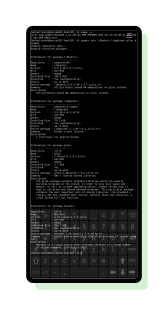
\includegraphics[height=1.0\textheight]{stack-lower}

\end{column}
\end{columns}

\end{frame}
\note{
}

%%%%%%%%%%%%%%%%%%%%%%%%%%%%%%%%%%%%%%%%%

\begin{frame}
\frametitle{Sailfish OS Stack}

\begin{columns}[T]
\begin{column}[T]{0.5\textwidth}
\setlength{\parskip}{0.5em}

\vspace{0.0cm}
\hspace{1.3cm}
\includegraphics[height=1.0\textheight]{stack-upper}

\end{column}
\begin{column}[T]{0.5\textwidth}
\setlength{\parskip}{0.5em}

\vspace{1.5cm}
\begin{enumerate}
\setcounter{enumi}{6}
\setlength{\parskip}{0.5em}
\item Qt middleware
\item Wayland + Lipstick compositor
\item Silica user interface
\item Lipstick launcher
\item Gecko-based Web browser
\item Android App Support
\end{enumerate}

\end{column}
\end{columns}

\end{frame}
\note{
}

%%%%%%%%%%%%%%%%%%%%%%%%%%%%%%%%%%%%%%%%%

\begin{frame}
\frametitle{Libhybris and Libgbinder}

\begin{columns}[T]
\begin{column}[T]{0.5\textwidth}
\setlength{\parskip}{0.5em}

\vspace{0.4cm}
Libhybris
\begin{enumerate}
\setlength{\parskip}{0.5em}
\item Allows AOSP drivers to be used with glibc Linux
\item Dynamic loading of Android libraries
\item Overrides bionic symbols with glibc symbols
\end{enumerate}

\end{column}
\begin{column}[T]{0.5\textwidth}
\setlength{\parskip}{0.5em}

\vspace{0.4cm}
Libgbinder
\begin{enumerate}
\setlength{\parskip}{0.5em}
\item Android Binder Protocol
\item HAL Interface definition language
\item Switching from linking to Binder
\item Modems switched from socket to Binder in Android 8
\end{enumerate}

\end{column}
\end{columns}

\end{frame}
\note{
}

%%%%%%%%%%%%%%%%%%%%%%%%%%%%%%%%%%%%%%%%%

\begin{frame}[fragile]
\frametitle{DBus}

\begin{columns}[T]
\begin{column}[T]{0.5\textwidth}
\setlength{\parskip}{0.5em}

\vspace{0.4cm}
Inter-process communication
\begin{enumerate}
\setlength{\parskip}{0.5em}
\item Object-oriented and typed
\item System bus, per-login session bus
\item Peer-to-peer or bus-oriented
\item Properties, method calls, signals, introspection
\end{enumerate}

\end{column}
\begin{column}[T]{0.5\textwidth}

\begin{lstlisting}[language=cpp]
class FlashlightDBusAdaptor: public QDBusAbstractAdaptor
{
    Q_OBJECT
    Q_CLASSINFO("D-Bus Interface",
        "com.jolla.settings.system.flashlight")

public:
    Q_PROPERTY(bool flashlightOn READ flashlightOn)

    FlashlightDBusAdaptor(QObject *parent);
    bool flashlightOn() const;

public slots:
    bool toggleFlashlight();

signals:
    void flashlightOnChanged();
};
\end{lstlisting}

\begin{lstlisting}[language=sh2]
dbus-send --session --type="method_call" --print-reply \
    --dest="com.jolla.settings.system.flashlight" \
    "/com/jolla/settings/system/flashlight" \
    "com.jolla.settings.system.flashlight.toggleFlashlight"
\end{lstlisting}

\end{column}
\end{columns}

\end{frame}
\note{
}

%%%%%%%%%%%%%%%%%%%%%%%%%%%%%%%%%%%%%%%%%

\begin{frame}[fragile]
\frametitle{Qt}

\begin{columns}[T]
\begin{column}[T]{0.5\textwidth}
\setlength{\parskip}{0.5em}

\vspace{1.0cm}
\begin{enumerate}
\setlength{\parskip}{0.5em}
\item Middleware libraries
\item User Interface toolkit
\item Cross-platform C++, PyOtherSide
\item Meta-Object Compiler
\item QObject model
\end{enumerate}

\end{column}
\begin{column}[T]{0.5\textwidth}

\begin{lstlisting}[language=cpp]
#include <QObject>

class Example : public QObject
{
    Q_OBJECT

    Q_PROPERTY(bool selected READ selected WRITE setSelected NOTIFY selectedChanged)
public:
    explicit Example(QObject *parent = nullptr)
        : QObject(parent)
        , m_selected(false)
    {}

    bool selected() const { return m_selected; }

    void setSelected(bool selected) {
        if (m_selected != selected) {
            m_selected = selected;
            emit selectedChanged();
        }
    }

signals:
    void selectedChanged();

private:
    bool m_selected;
};
\end{lstlisting}
\end{column}
\end{columns}

\end{frame}
\note{
}

%%%%%%%%%%%%%%%%%%%%%%%%%%%%%%%%%%%%%%%%%

\begin{frame}[fragile]
\frametitle{QML}

\begin{columns}[T]
\begin{column}[T]{0.5\textwidth}
\setlength{\parskip}{0.5em}

\vspace{1.0cm}
\begin{enumerate}
\setlength{\parskip}{0.5em}
\item Declarative user interface language
\item {\it Components\/}, {\it properties\/} and {\it functions\/}
\item Property changes trigger recalculation
\item Imperative JavaScript functions
\item Rendered components positioned using anchors
\end{enumerate}

\end{column}
\begin{column}[T]{0.5\textwidth}

\vspace{-0.2cm}
\begin{lstlisting}[language=QML]
Page {
    property int count: 0

    Example {
        id: example
        selected: toggle.checked
    }

    Timer {
        id: countdown; interval: 1000; repeat: true
        onTriggered: if (count > 0) count -= 1
        running: example.selected == true
        onRunningChanged: count = 10
    }

    Column {
        id: column; anchors.fill: parent
        PageHeader { title: qsTr("REG Tech Talk Example") }
        TextSwitch {
            id: toggle
            text: qsTr("Activated")
        }

        Label {
            x: Theme.horizontalPageMargin
            text: example.selected
                  ? qsTr("This message will self destruct in %1 seconds".arg(count))
                  : qsTr("Disarmed")
        }
    }
}
\end{lstlisting}
\end{column}
\end{columns}

\end{frame}
\note{
}

%%%%%%%%%%%%%%%%%%%%%%%%%%%%%%%%%%%%%%%%%

\begin{frame}[fragile]
\frametitle{Hacking the Homescreen}

\begin{columns}[T]
\begin{column}[T]{1.0\textwidth}
\setlength{\parskip}{0.5em}

\vspace{0.4cm}
\begin{enumerate}
\setlength{\parskip}{0.5em}
\item QML interface is highly hackable
\item A simple example:
\end{enumerate}

{\tt /usr/share/lipstick-jolla-home-qt5/statusarea/StatusArea.qml}
\vspace{0.2cm}
\begin{lstlisting}[language=QML,firstnumber=141]
            Label {
                id: name
                text: "David's phone"
                anchors.verticalCenter: parent.verticalCenter
            }
\end{lstlisting}



\end{column}
\end{columns}

\end{frame}
\note{
}

%%%%%%%%%%%%%%%%%%%%%%%%%%%%%%%%%%%%%%%%%

\begin{frame}
\frametitle{Sailfish SDK}

\begin{columns}[T]
\begin{column}[T]{0.5\textwidth}
\setlength{\parskip}{0.5em}

\vspace{0.3cm}
\hspace{0.1cm}
\includegraphics[width=0.9\textwidth]{sailfishide}

\end{column}
\begin{column}[T]{0.5\textwidth}
\setlength{\parskip}{0.5em}

\vspace{0.3cm}
\includegraphics[width=0.9\textwidth]{sfdk}

\end{column}
\end{columns}

\end{frame}
\note{
}

%%%%%%%%%%%%%%%%%%%%%%%%%%%%%%%%%%%%%%%%%

\begin{frame}
\frametitle{Android App Support}

\begin{columns}[T]
\begin{column}[T]{1.0\textwidth}
\setlength{\parskip}{0.5em}

\begin{column}[T]{1.0\textwidth}

\vspace{0.5cm}
\includegraphics[width=1.0\textwidth]{aas}

\end{column}

\end{column}
\end{columns}

\end{frame}
\note{
}

%%%%%%%%%%%%%%%%%%%%%%%%%%%%%%%%%%%%%%%%%

\begin{frame}
\frametitle{Is it Open Source?}

\begin{columns}[T]
\begin{column}[T]{0.5\textwidth}
\setlength{\parskip}{0.5em}

\vspace{0.4cm}
Closed drivers, everything else open
\begin{enumerate}
\setlength{\parskip}{0.5em}
\item Mobian
\item postmarketOS
\item Ubuntu Touch
\item Nemo Mobile
\end{enumerate}

\end{column}
\begin{column}[T]{0.5\textwidth}
\setlength{\parskip}{0.5em}

\vspace{0.4cm}
Sailfish OS
\begin{enumerate}
\setlength{\parskip}{0.5em}
\item Closed drivers
\item Linux kernel open
\item Middleware, Qt open
\item User interface closed
\item Jolla apps closed
\item Android App Support closed
\end{enumerate}

\end{column}
\end{columns}

\end{frame}
\note{
}

%%%%%%%%%%%%%%%%%%%%%%%%%%%%%%%%%%%%%%%%%

\begin{frame}
\frametitle{Exciting Community Projects}

\begin{columns}[T]
\begin{column}[T]{0.5\textwidth}
\setlength{\parskip}{0.5em}

\vspace{1.0cm}
Lots of neat stuff...
\begin{enumerate}
\setlength{\parskip}{0.5em}
\item Flatpack support
\item Sailfish on x86
\item AsteroidOS
\item SDK Rust support
\end{enumerate}

\end{column}

\begin{column}[T]{0.5\textwidth}
\setlength{\parskip}{0.5em}

\vspace{0.5cm}
\includegraphics[width=0.7\textwidth]{asteroidos}

\end{column}
\end{columns}

\end{frame}
\note{
}

%%%%%%%%%%%%%%%%%%%%%%%%%%%%%%%%%%%%%%%%%

\begin{frame}
\frametitle{Supported Devices}

\begin{columns}[T]
\begin{column}[T]{1.0\textwidth}
\setlength{\parskip}{0.5em}



\rowcolors{1}{gray!15}{white}
\begin{tabular}{L{1.5cm}|L{3cm}|L{4.5cm}|L{2.7cm}} \hline
\rowcolor{blue!25}
{\bf Distribution} & {\bf Official} & {\bf Community} & {\bf More info} \\ \hline
Sailfish OS & Xperia X, XA2, 10, 10 II, 10 III, Gemini & PinePhone, Fairphone 2, Galaxy Note 4, F(x)Tec Pro, Volla, plus at least 20 others & \href{https://forum.sailfishos.org/t/community-hardware-adaptations/14081}{forum.sailfishos.org/t/14081} \\
Mobian & PinePhone, Librem 5, OnePlus 6/6T, Pocophone F1 & Fairphone 4, SHIFT6mq, Mi Mix 2S & \href{https://wiki.mobian.org/?id=devices}{wiki.mobian.org/?id=devices} \\
postmarketOS & PinePhone, Librem 5 & Fairphone 4, OnePlus 6/6T, Galaxy A3/A5/E7/Tab, Pocophone F1, Mi Note 2, plus at least 20 more & \href{https://postmarketos.org/download/}{postmarketos.org/download} \\
Ubuntu Touch & Volla, Fairphone 2, Nexus 5, OnePlus One, PinePhone & Pixel 3a, Poco X3, Mi A2, BQ Aquaris M10, Asus Zenfone Max Pro M1, Xperia X & \href{https://devices.ubuntu-touch.io/}{devices.ubuntu-touch.io} \\
Nemo Mobile & PinePhone, Volla & -- & \href{https://nemomobile.net/devices/}{nemomobile.net/devices} \\ \hline
\end{tabular}


\end{column}
\end{columns}

\end{frame}
\note{
}

%%%%%%%%%%%%%%%%%%%%%%%%%%%%%%%%%%%%%%%%%

\begin{frame}[fragile]
\frametitle{PyTorch Lightning}

\begin{columns}[T]
\begin{column}[T]{0.5\textwidth}
\setlength{\parskip}{0.5em}

\vspace{0.6cm}
\begin{lstlisting}[language=sh]
zypper install gcc python3-devel
python3 -m venv venv
. ./venv/bin/activate
python3 -m pip install torch lightning torchvision
python3 example.py
\end{lstlisting}

\vspace{0.2cm}
\begin{lstlisting}[language=python]
# See: https://lightning.ai/docs/pytorch/stable/starter/introduction.html

import os
from torch import optim, nn, utils, Tensor
from torchvision.datasets import MNIST
from torchvision.transforms import ToTensor
import lightning.pytorch as pl

# define any number of nn.Modules (or use your current ones)
encoder = nn.Sequential(nn.Linear(28 * 28, 64), nn.ReLU(), nn.Linear(64, 3))
decoder = nn.Sequential(nn.Linear(3, 64), nn.ReLU(), nn.Linear(64, 28 * 28))

# define the LightningModule
class LitAutoEncoder(pl.LightningModule):
    def __init__(self, encoder, decoder):
        super().__init__()
        self.encoder = encoder
        self.decoder = decoder
\end{lstlisting}

\end{column}
\begin{column}[T]{0.5\textwidth}
\setlength{\parskip}{0.5em}

\vspace{0.6cm}
\begin{lstlisting}[language=python,firstnumber=20]
    def training_step(self, batch, batch_idx):
        # training_step defines the train loop.
        # it is independent of forward
        x, y = batch
        x = x.view(x.size(0), -1)
        z = self.encoder(x)
        x_hat = self.decoder(z)
        loss = nn.functional.mse_loss(x_hat, x)
        # Logging to TensorBoard (if installed) by default
        self.log("train_loss", loss)
        return loss

    def configure_optimizers(self):
        optimizer = optim.Adam(self.parameters(), lr=1e-3)
        return optimizer

# init the autoencoder
autoencoder = LitAutoEncoder(encoder, decoder)

# setup data
dataset = MNIST(os.getcwd(), download=True, transform=ToTensor())
train_loader = utils.data.DataLoader(dataset, num_workers=4)

# train the model (hint: here are some helpful Trainer arguments for rapid idea iteration)
trainer = pl.Trainer(limit_train_batches=100, max_epochs=1)
trainer.fit(model=autoencoder, train_dataloaders=train_loader)

\end{lstlisting}

\end{column}
\end{columns}

\end{frame}
\note{
}

%%%%%%%%%%%%%%%%%%%%%%%%%%%%%%%%%%%%%%%%%

\begin{frame}[fragile]
\frametitle{Jupyter Lab}

\begin{columns}[T]
\begin{column}[T]{0.5\textwidth}
\setlength{\parskip}{0.5em}

\vspace{3.0cm}
\begin{lstlisting}[language=sh]
python3 -m venv venv-jupyter
. ./venv-jupyter/bin/activate
pip install jupyter ipykernel matplotlib
python3 -m ipykernel install --user --name=venv-jupyter
jupyter notebook password
jupyter notebook --ip 10.0.0.42 --port 8888
\end{lstlisting}

\end{column}
\begin{column}[T]{0.5\textwidth}
\setlength{\parskip}{0.5em}

\vspace{0.0cm}
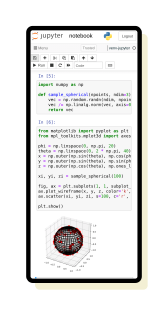
\includegraphics[height=1.0\textheight]{jupyter}

\end{column}
\end{columns}

\end{frame}
\note{
}

%%%%%%%%%%%%%%%%%%%%%%%%%%%%%%%%%%%%%%%%%

\begin{frame}[fragile]
\frametitle{Further info}
\setlength{\leftmargini}{7.0em}
\vspace{0.8cm}

\begin{itemize}
\setlength{\parskip}{1.0em}
\item[Sailfish OS] \, \url{https://sailfishos.org}
\item[Ubuntu Touch] \, \url{https://ubports.com}
\item[postmarketOS] \, \url{https://postmarketos.org}
\item[Mobian] \, \url{https://mobian-project.org}
\item[Nemo Mobile] \, \url{https://nemomobile.net}
\item[Slides source] \, \url{https://github.com/llewelld/reg-tech-talk-linux}
\end{itemize}

\end{frame}
\note{
\fontsize{7pt}{8pt}{\bibliographystyle{ieeetr}}
\bibliography{slides}

{\tiny Tux image attribution: lewing@isc.tamu.edu Larry Ewing and The GIMP}
}

%%%%%%%%%%%%%%%%%%%%%%%%%%%%%%%%%%%%%%%%%

\end{document}
